\chapter{The O'Briens in Boston}

The O'Briens\index{O'Brien!family} were among the almost 1.5 million Irish who sailed to the United States between 1845 and 1855.\cite{Miller:291} William\textsuperscript{1}'s\index{O'Brien!William\textsuperscript{1}} two youngest children, Michael\textsuperscript{2}\index{O'Brien!Michael\textsuperscript{2}} and Mary\textsuperscript{2},\index{O'Brien!Mary\textsuperscript{2}}\index{Ward!Mary\textsuperscript{2} (O'Brien)} were likely the first of the O'Brien family\index{O'Brien!family} to make the voyage. Irish families often could only afford tickets for one or two people, and so would choose the youngest and healthiest children.\cite{Miller:292} Once in America, the children would send remittances back to Ireland\index{Ireland} until the rest of the family could be brought over.\cite{Miller:295}

\begin{figure}
	\centering
	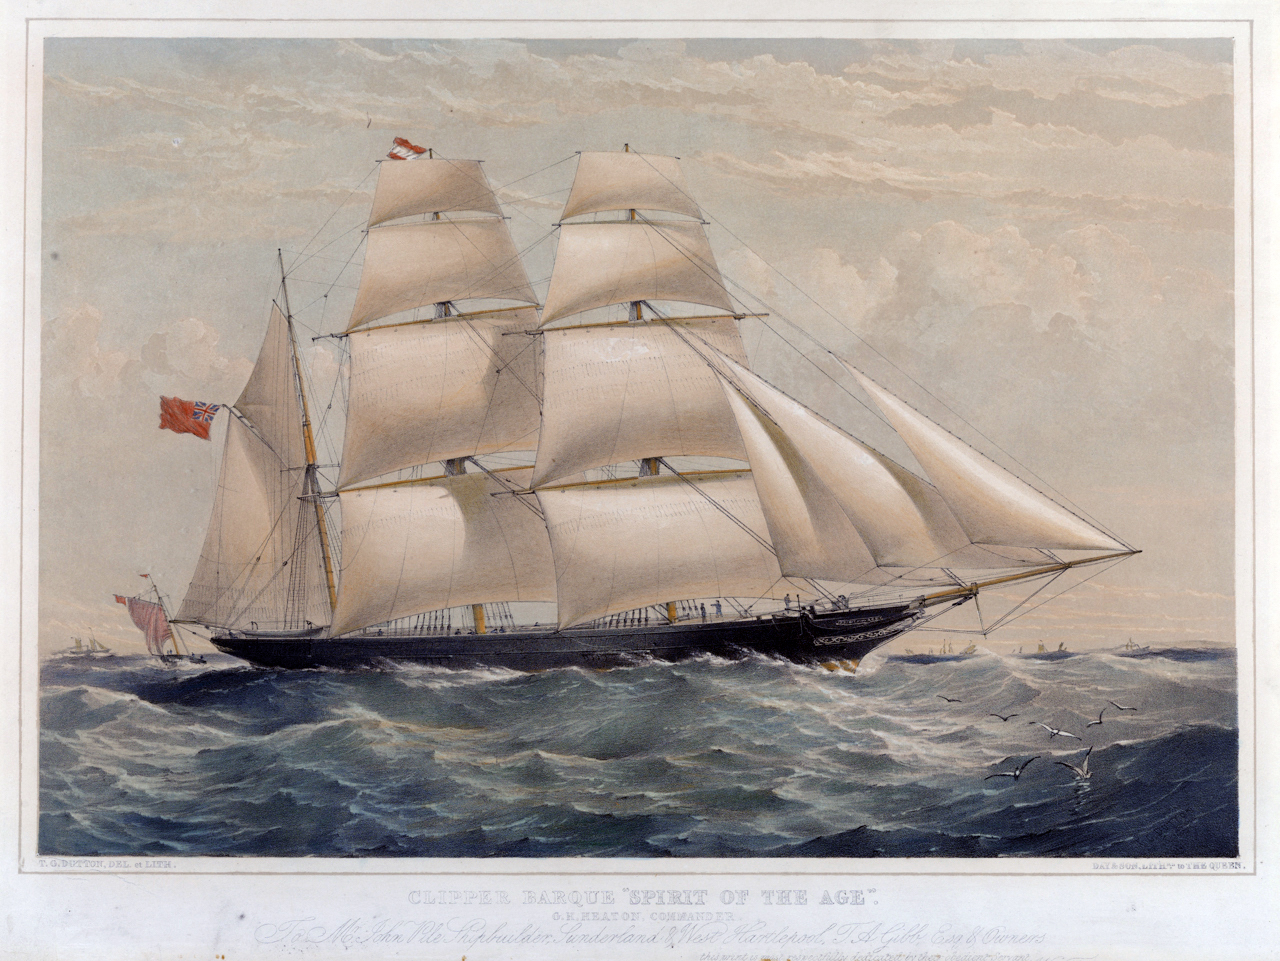
\includegraphics[width=\textwidth]{clipper_barque}
	\caption{Example of a clipper barque\index{clipper barque/bark} from 1854.}
	\label{fig:Clipper}
\end{figure}

\begin{figure}
	\centering
	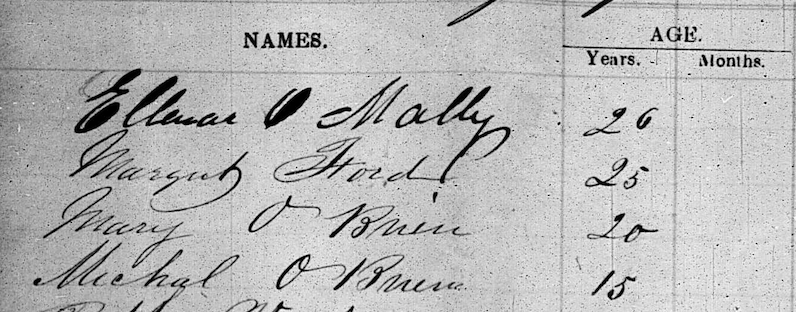
\includegraphics[width=\textwidth]{mary_michael}
	\caption{Passenger list of the \textit{Thomas Baker}\index{Thomas Baker (ship)} showing Mary O'Brien\index{O'Brien!Mary\string\textsuperscript{2}}\index{Ward!Mary\string\textsuperscript{2} (O'Brien)} and Michael O'Brien.\index{O'Brien!Michael\string\textsuperscript{2}}}
	\label{fig:ThomasBaker}
\end{figure}

\begin{figure}
	\centering
	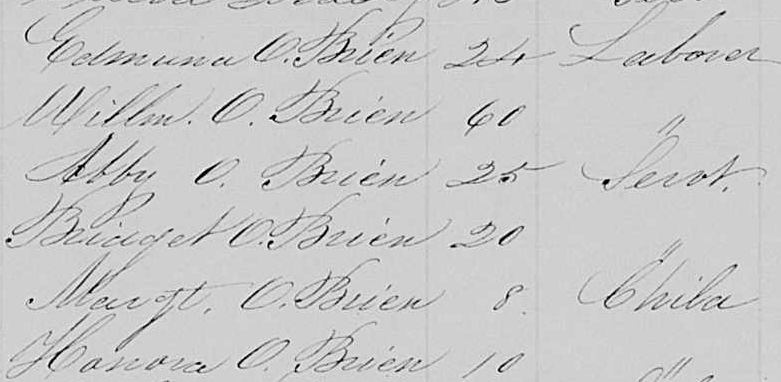
\includegraphics[width=\textwidth]{edward_ship}
	\caption{Passenger list of the \textit{Chasca}\index{Chasca (ship)} showing O'Brien family\index{O'Brien!family} along with ages and occupations.}
	\label{fig:Chasca}
\end{figure}

Ship passenger lists for the Port of New York\index{New York City} show a Mary O'Brien,\index{O'Brien!Mary\textsuperscript{2}}\index{Ward!Mary\textsuperscript{2} (O'Brien)} age 20, and Michael O'Brien,\index{O'Brien!Michael\textsuperscript{2}} age 15, arriving on the brig \textit{Thomas Baker}\index{Thomas Baker (ship)} from Galway, Ireland,\index{Ireland!Galway (city)} on 3 July 1849. There were 93 total passengers aboard. The occupation listed for everyone on the passenger manifest is ``farming.''\index{farming}\cite{ThomasBaker}

Brigs\index{Brigs} like the \textit{Thomas Baker}\index{Thomas Baker (ship)} were two-masted ships with square sails.\cite{OHanlon:35} Prior to the famine,\index{famine} these ships were outfitted for cargo rather than passengers.\cite{Laxton:9} The \textit{Thomas Baker},\index{Thomas Baker (ship)} for instance, was a coal-hauling ship.\cite{MorningAdvertiser} Compared to the three-masted liners, brigs\index{Brigs} were cramped for the number of passengers they carried, with poor ventilation and five-foot ceilings.\cite{OHanlon:33} The voyage from Ireland\index{Ireland} to the United States took anywhere from four to eight weeks.

A larger group of the O'Briens\index{O'Brien!family} arrived in Boston on 27 June 1851 on board the vessel \textit{Chasca}\cite{Chascay:1}.\index{Chasca (ship)} The voyage from Liverpool, England,\index{England!Liverpool} to Boston, Massachusetts,\index{Massachusetts!Boston} took 47 days.\cite{Chascay2:1} On board were Edward\textsuperscript{2} O'Brien\index{O'Brien!Edward/Edmund\textsuperscript{2}} (appearing as Edmund\footnote{Edward is also named as Edmund in daughter Mary Ann O'Brien's birth record. By the time his second child Ellen was born, he was going by Edward.}), his father William,\index{O'Brien!William\textsuperscript{1}} wife Bridget\index{Linehan/Linnehan!Bridget}\index{O'Brien!Bridget (Linnehan)}, sister Abby\textsuperscript{2} (O'Brien) Dooley,\index{O'Brien!Abigail\textsuperscript{2}}\index{Dooley!Abigail\textsuperscript{2} (O'Brien)} and Abby's two children, Margaret\textsuperscript{3}\index{Dooley!Margaret\textsuperscript{3}}\index{Fernald!Margaret\textsuperscript{3} (Dooley) (Simonds)}\index{Simonds!Margaret\textsuperscript{3} (Dooley)} and Hanora\textsuperscript{3} (aka Hannah).\index{Dooley!Hannah/Hanora\textsuperscript{3}}\index{Cooney!Hannah/Hanora\textsuperscript{3} (Dooley)}\index{Cusick!Hannah/Hanora\textsuperscript{3} (Dooley) (Cooney)} There were a total of 256 passengers on board,\cite{Chascay:2} which must have made the ship quite crowded. The \textit{Chasca}\index{Chasca (ship)} was a 658-ton clipper bark\index{clipper barque/bark} built in East Boston\index{Massachusetts!Boston!East Boston} as a speedy cargo ship\cite{ChascaCard,Chascay:3} Like the \textit{Thomas Baker}\index{Thomas Baker (ship)}, it was probably retrofitted to carry passengers in response to the large demand for transport to the New World during the famine\index{famine} years.

Both Abby's\index{Dooley!Abigail\textsuperscript{2} (O'Brien)}\index{O'Brien!Abigail\textsuperscript{2}} and Margaret's\index{Dooley!Margaret\textsuperscript{3}}\index{Fernald!Margaret\textsuperscript{3} (Dooley) (Simonds)}\index{Simonds!Margaret\textsuperscript{3} (Dooley)} occupations are listed as ``Servt.''\index{servant} in the passenger manifest.\cite{Chascay:4} About 2,000 Irish women\index{Irish-Americans} in Boston\index{Massachusetts!Boston} were domestic workers\index{Domestic workers} in 1850. It was a popular trade for Irish\index{Irish-Americans} immigrant women since they spoke English and didn't have many other opportunities for work available to them.\cite{Ryan:41}

William's\index{O'Brien!William\textsuperscript{1}} remaining two children, John\textsuperscript{2}\index{O'Brien!John\textsuperscript{2}} and Ann\textsuperscript{2},\index{O'Brien!Ann\textsuperscript{2}}\index{Dailey!Ann\textsuperscript{2} (O'Brien)} made separate voyages from Ireland\index{Ireland} to Boston\index{Massachusetts!Boston} but cannot be found in passenger records. John\index{O'Brien!John\textsuperscript{2}} must have arrived sometime prior to his marriage in 1853.\cite{John2OBrienCivilMarriage:1} Ann\index{O'Brien!Ann\textsuperscript{2}}\index{Dailey!Ann\textsuperscript{2} (O'Brien)} may not have arrived until 1870--1880 as she doesn't appear in any prior records.\cite{Census1880Edward:1} 

Like other Irish\index{Irish-Americans} immigrants from this time period, William O'Brien\index{O'Brien!William\textsuperscript{1}} and his children likely came to America to escape the famine\index{famine} and build a better life. While the family may have avoided starvation in Ireland,\index{Ireland} the first few years in Boston\index{Massachusetts!Boston} presented new challenges. The O'Briens\index{O'Brien!family} lived in crowded tenement buildings, suffered devastating losses from communicable diseases, and likely faced anti-Catholic\index{Catholicism} discrimination from the city's dominant class of Protestants.\index{Protestantism}\cite{Ryan:61,Quinlan:58}
	
Moving frequently at first, the family lived predominantly in Boston's North End\index{Massachusetts!Boston!North End} neighborhood during the 1850s and 1860s.\cite{NorthEndAddresses} In 1855, half of all residents of the North End\index{Massachusetts!Boston!North End} were Irish.\index{Irish-Americans}\cite{Todisco:29} Landlords had subdivided the North End's old mansions and warehouses into crowded tenement houses for renting to the newly-arrived immigrants.\cite{Goldfeld:102} Many of the tenements were not connected to sewage systems or had defective toilets, leading to high rates of infant mortality and diseases like smallpox, cholera, and tuberculosis.\cite{Goldfeld:103,Todisco:21,Ryan:48}

In 1834, Irish immigrants\index{Irish-Americans} founded the first Catholic church\index{Catholicism} in Boston's North End\index{Massachusetts!Boston!North End} --- St.\ Mary's of the Sacred Heart,\index{St.\ Mary's of the Sacred Heart (church)} on the corner of Endicott\index{Massachusetts!Boston!Endicott St.} and Cooper Streets.\index{Massachusetts!Boston!Cooper St.}\cite{Todisco:26} John O'Brien\index{O'Brien!John\textsuperscript{2}} married Mary Mahony\index{Mahoney/Mahony!Mary}\index{O'Brien!Mary (Mahoney)}\index{Bowser!Mary (Mahoney) (O'Brien)} there in 1853.\cite{John2OBrienMarriage:1} St.\ Mary's\index{St.\ Mary's of the Sacred Heart (church)} quickly reached capacity, and so in 1843, St.\ John the Baptist Church\index{St.\ John the Baptist (church)} was founded in a converted pork storehouse on Moon St.\index{Massachusetts!Boston!Moon St.}\cite{Goldfeld:101,Sullivan:128:1} John's children Mary\textsuperscript{3}\index{O'Brien!Mary\textsuperscript{3} (1856--1883)} and Ellen\textsuperscript{3}\index{O'Brien!Ellen/Nellie\textsuperscript{3} (1859--1882)} were baptized there. St.\ John's,\index{St. John the Baptist (church)} too, became crowded, which in 1862 lead to the Catholics\index{Catholicism} purchasing the New North Church\index{New North Church} at the corner of Hanover\index{Massachusetts!Boston!Hanover St.} and Clark Streets\index{Massachusetts!Boston!Clark St.} and re-dedicating it as St.\ Stephen's.\index{St. Stephen's (church)}\cite{Sullivan:128:2} The O'Brien family\index{O'Brien!family} followed many other Irish\index{Irish-Americans} in moving from St.\ John's\index{St. John the Baptist (church)} to St.\ Stephen's\index{St. Stephen's (church)} when it opened. The O'Briens' baptisms and marriages took place at St.\ Stephen's\index{St. Stephen's (church)} at least until Margaret Dooley's\index{Dooley!Margaret\textsuperscript{3}}\index{Fernald!Margaret\textsuperscript{3} (Dooley) (Simonds)}\index{Simonds!Margaret\textsuperscript{3} (Dooley)} marriage there in 1873.\cite{RobertFernaldMarriage:1}

\begin{figure}
	\centering
	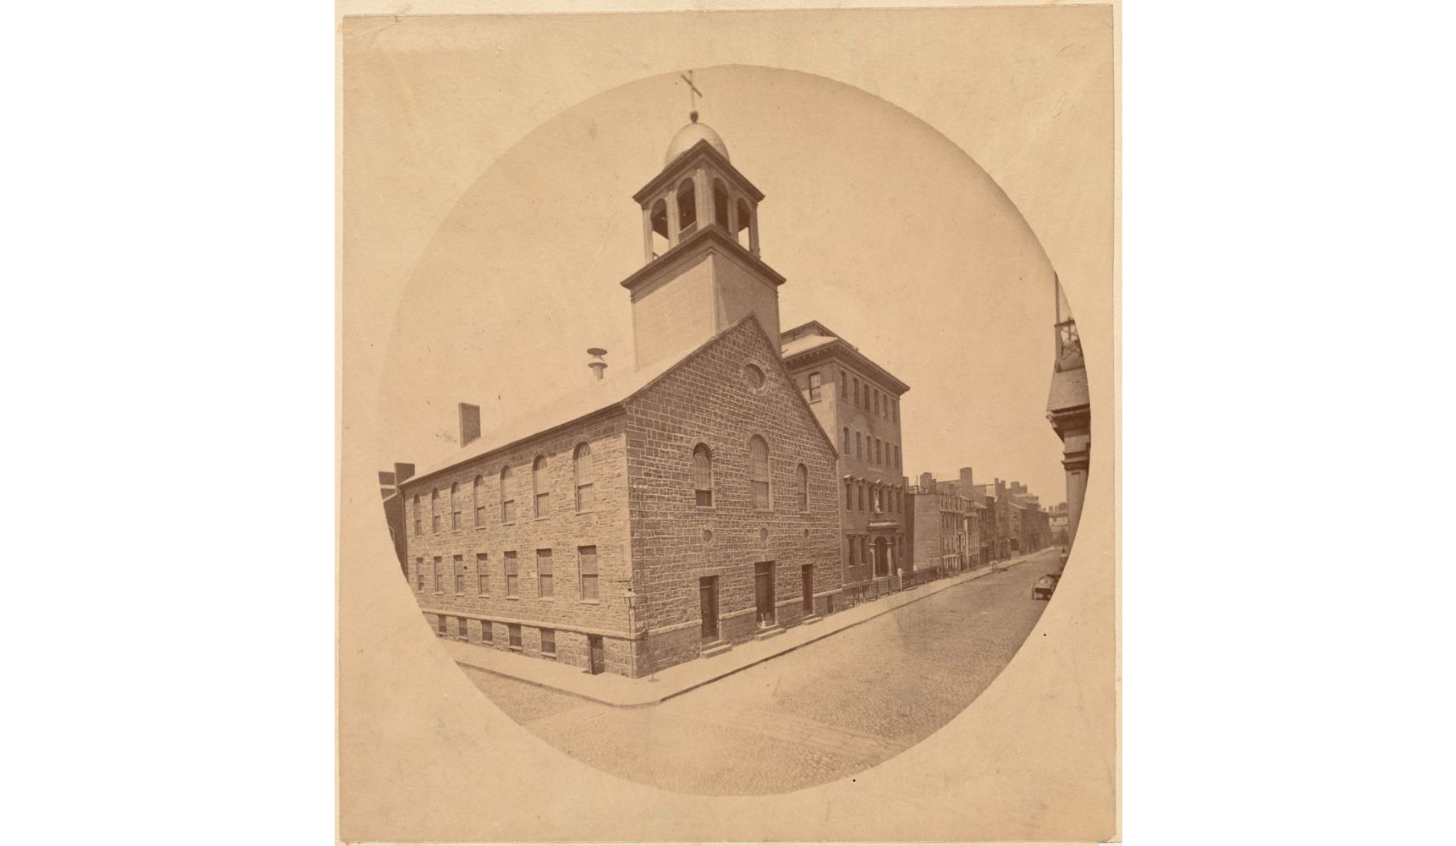
\includegraphics[width=\textwidth]{st_marys}
	\caption{St. Mary's of the Sacred Heart Church}
	\label{fig:StMarys}
\end{figure}

Irish\index{Irish-Americans} immigrants to Boston\index{Massachusetts!Boston} had difficulty finding steady work, given that they were mostly rural farmers\index{farming} and did not have specialized trade skills.\cite{Ryan:21} Many of them started out by opening a grocery\index{grocer} store in their tenement house or somewhere close by.\cite{Ryan:83} Indeed, John's\index{O'Brien!John\textsuperscript{2}} occupation is listed as ``grocer''\index{grocer} on his son John Joseph's\index{O'Brien!John Joseph\textsuperscript{3} (1861--1938)} birth record.\cite{John3OBrienBirth:1} 

John\index{O'Brien!John\textsuperscript{2}} and his brother Michael\index{O'Brien!Michael\textsuperscript{2}} both worked as oystermen.\index{oyster harvesting}\cite{EdwardFrancis3OBrienBirth:1,Michael2OBrien1886:1,1861John2OBrien:1} Before the advent of industrial-scale dredging operations, the traditional method of oyster harvesting\index{oyster harvesting} used tongs. Oyster tongs consisted of a pair of metal rakes at the end of long wooden shafts. The oysterman\index{oyster harvesting} would use the tongs to scrape oysters off the bottom of the sea bed and manually haul them onto the boat, up to 70 pounds at a time. The boats were small vessels rigged with one or two sails.\cite{Botwick:95} Being an oysterman\index{oyster harvesting} brought a degree of independence for an unskilled laborer. He typically owned his own boat and tackle, shucked the oysters at home to sell locally, and kept all the profits.\cite{MacKenzie:7:1, Botwick:96} This changed beginning in the 1870s when steam-powered oyster dredging ships arrived, and packing houses took over the oyster shucking process.\cite{MacKenzie:5, MacKenzie:7:2} 

The natural oyster beds in the Charles and Mystic Rivers had long been depleted by the time the O'Briens arrived in Boston. Even the oysters around Cape Cod and Rhode Island were diminishing. The Boston oyster dealers replaced the naturally-growing oysters with seed oysters from Long Island Sound and New Jersey at first, and eventually from Virginia, ``planting'' them in the spring and then harvesting the fully-grown oysters in the fall and winter. Ships would bring the oysters into Boston from Wellfleet on Cape Cod, or other planted beds in Narragansett and Buzzard's Bays. Sailors unloaded the oysters at the docks near Fanueil Hall and sold them to local dealers and peddlers.\cite{Ingersoll:27-28} 

Oyster shuckers worked seasonally from September to May. It was a difficult, low-paying job. In 1880 they were paid between 17 and 20 cents per gallon of oysters shucked. Steamships began bringing twice-weekly shipments of opened oysters to Boston from Norfolk, Virginia, making it more difficult to find local employment in the oyster trade.\cite{Ingersoll:30}

\begin{figure}
	\centering
	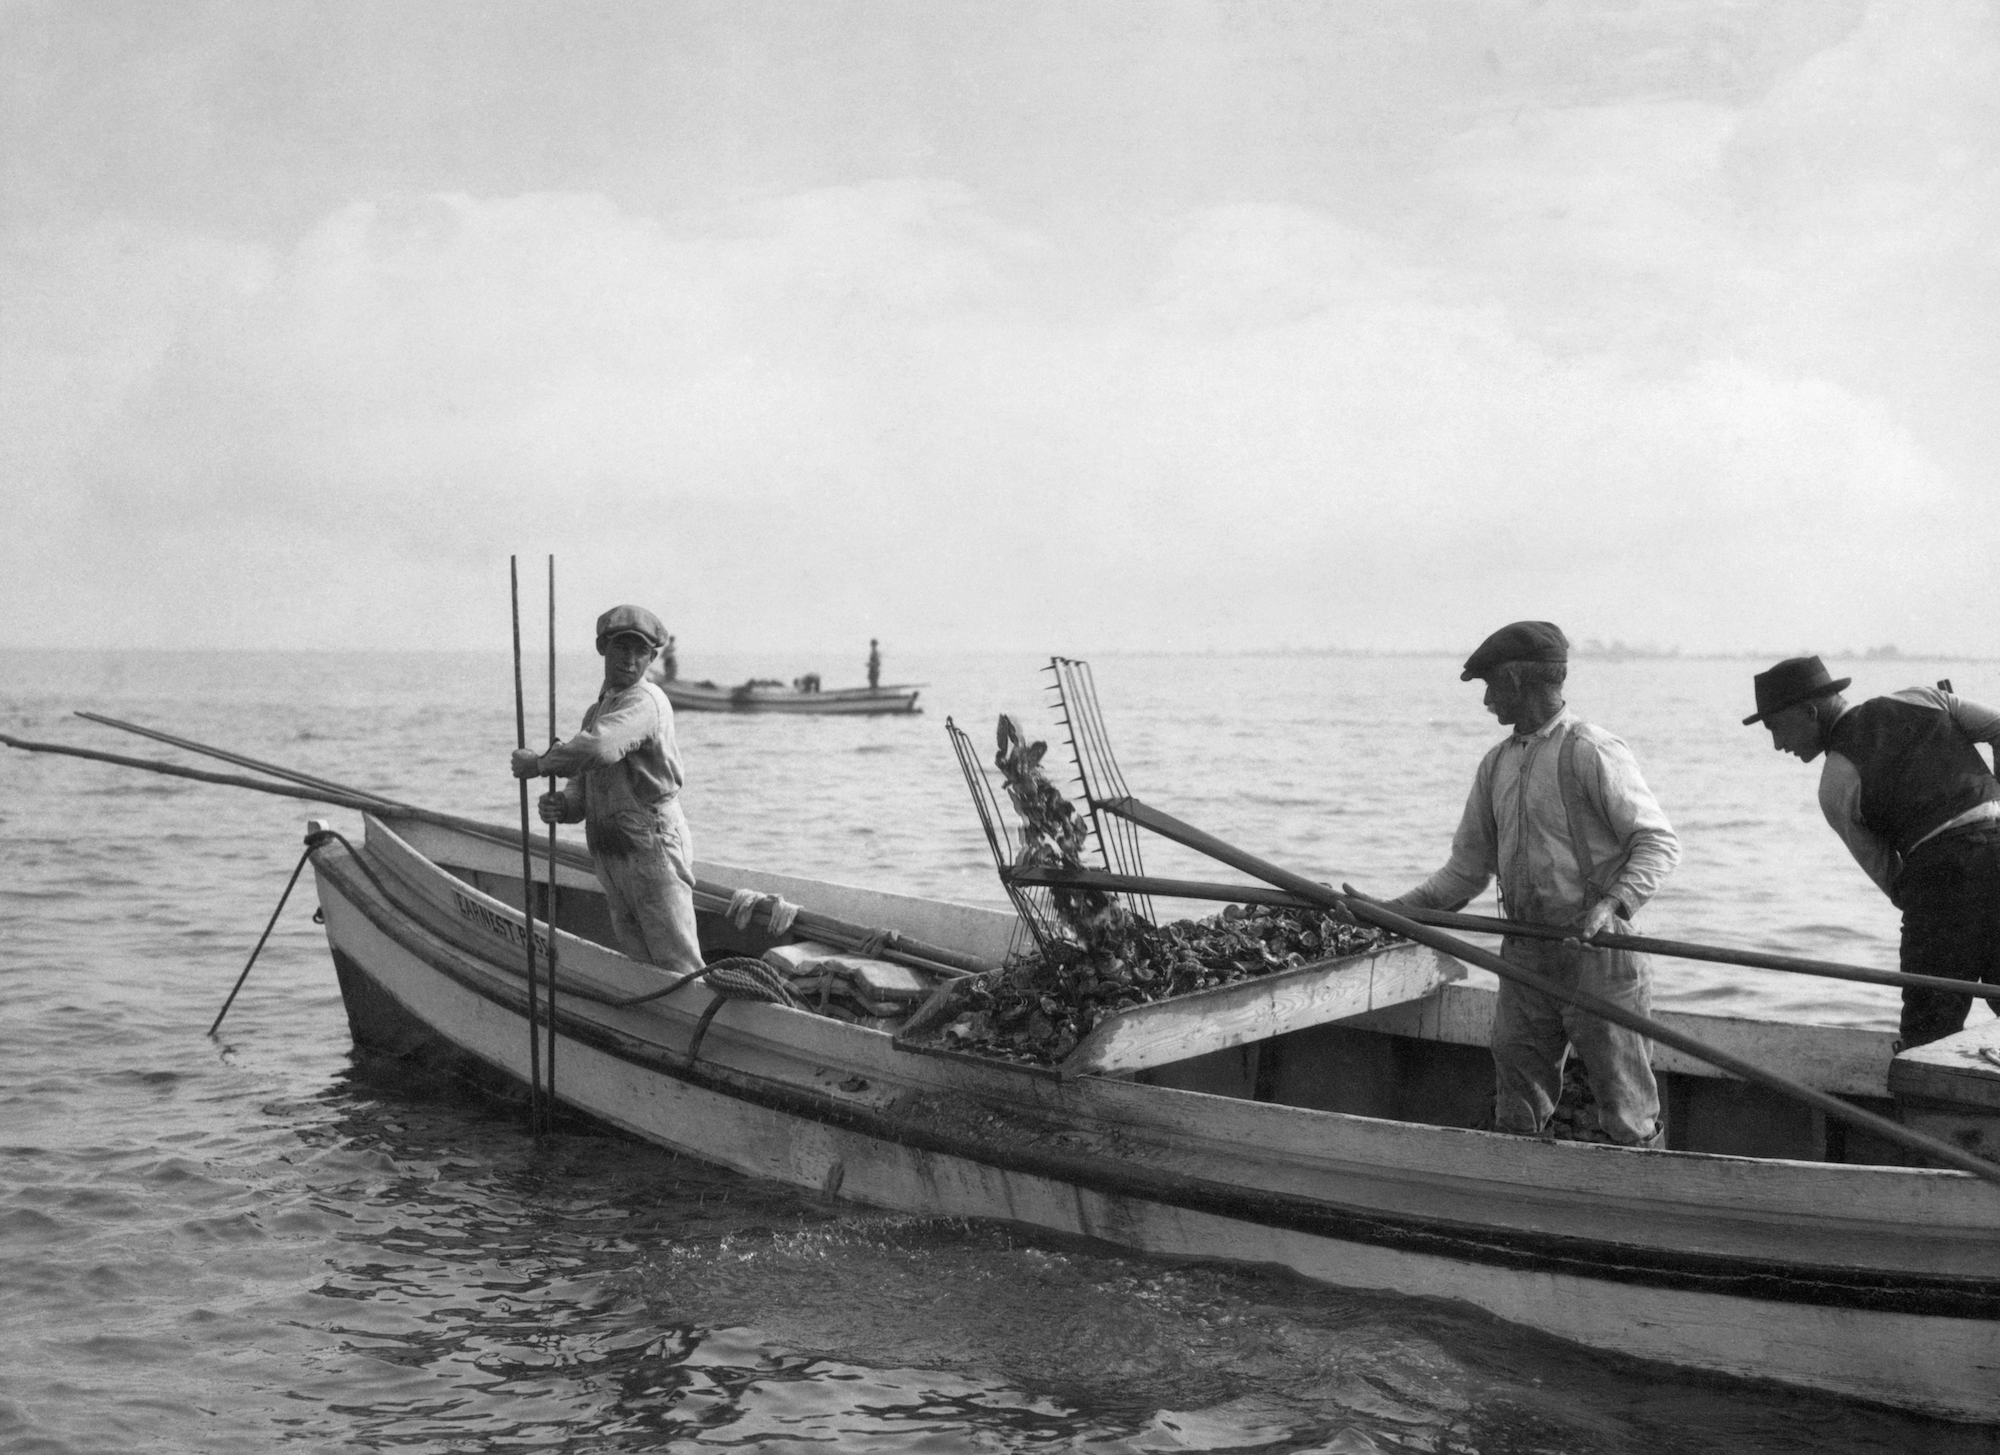
\includegraphics[width=\textwidth]{NatGeo_1238550}
	\caption{Oyster tongers}\index{oyster harvesting}
	\label{fig:OysterTongers}
\end{figure}

It seems that Edward\index{O'Brien!Edward/Edmund\textsuperscript{2}} was the main provider for the O'Brien family\index{O'Brien!family} during the early years in Boston.\index{Massachusetts!Boston} He may have had a successful trade in Ireland\index{Ireland} prior to his arrival in the United States. In 1855 he was housing his father and his sister Abby's\index{Dooley!Abigail\textsuperscript{2} (O'Brien)}\index{O'Brien!Abigail\textsuperscript{2}} family in addition to his own.\cite{Census1855William:1} Edward\index{O'Brien!Edward/Edmund\textsuperscript{2}} purchased a 2-person cemetery plot at North Cambridge Catholic Cemetery\index{North Cambridge Catholic Cemetery} in 1852\cite{CarolGordon:1} and a large 13-person plot at Holy Cross Cemetery\index{Holy Cross Cemetery} in 1880\cite{HolyCrossPlotEdward:1} where many of his family members were buried.

In the early 1870s, most of William's\index{O'Brien!William\textsuperscript{1}} adult children (Edward,\index{O'Brien!Edward/Edmund\textsuperscript{2}} Ann,\index{O'Brien!Ann\textsuperscript{2}}\index{Dailey!Ann\textsuperscript{2} (O'Brien)} Mary,\index{O'Brien!Mary\textsuperscript{2}}\index{Ward!Mary\textsuperscript{2} (O'Brien)} and Michael\index{O'Brien!Michael\textsuperscript{2}}) relocated to East Boston.\index{Massachusetts!Boston!East Boston} John's\index{O'Brien!John\textsuperscript{2}} sons, John Joseph\textsuperscript{3},\index{O'Brien!John Joseph\textsuperscript{3} (1861--1938)} James Edward\textsuperscript{3},\index{O'Brien!James Edward\textsuperscript{3}} and William\textsuperscript{3},\index{O'Brien!William\textsuperscript{3}} moved to Boston's South Cove\index{Massachusetts!Boston!South Cove} neighborhood (now part of Chinatown\index{Massachusetts!Boston!Chinatown}).\cite{1870sAddresses}

John's\index{O'Brien!John\textsuperscript{2}} family was hit particularly hard by tuberculosis.\index{tuberculosis}\index{phthisis|see{tuberculosis}}\index{consumption|see {tuberculosis}}\footnote{The terms ``phthisis'' and ``consumption'' were used at the time to describe what is now called tuberculosis.\cite{TuberculosisHistory}} Four of his children died of the disease between 1879 and 1889, as did John\index{O'Brien!John\textsuperscript{2}} himself in 1863.\cite{John2OBrienDeath:1} In fact, John's line would have ended if not for his son John Joseph.\index{O'Brien!John Joseph\textsuperscript{3} (1861--1938)} Tuberculosis\index{tuberculosis} disproportionately affected Irish immigrants\index{Irish-Americans} in Boston:\index{Massachusetts!Boston}

\begin{quote}
	\ldots[t]he death rate from consumption\index{tuberculosis} was greatest among the colored, and among the white \ldots it was greatest among those whose mothers were born in Ireland\index{Ireland}\index{Irish-Americans} or who were themselves natives of Ireland, being more than 3 times the corresponding rate for those whose mothers were born in the United States, and almost double the rate for those who were themselves natives of this country.\cite{VitalStatistics}
\end{quote}

Three of Michael's\index{O'Brien!Michael\textsuperscript{2}} sons had jobs working in Boston's\index{Massachusetts!Boston} gas industry.\index{gas industry} Their roles included gas meter maker, meter tester, meter reader, and foreman. The Boston Gas Company\index{Boston Gas Company} constructed a large coal gas plant at Commercial Point\index{Massachusetts!Boston!Commercial Point} in 1882. The company needed to hire a large number of unskilled laborers, and many of them were Irish\index{Irish-Americans} immigrants.\cite{Keating:11} In the early 20th century, these jobs were highly valued, as the company (later called Boston Consolidated Gas)\index{Boston Consolidated Gas} offered employee profit-sharing plans in 1906 and a pension plan in 1919. This provided job stability and wealth for the Irish\index{Irish-Americans} working class.\cite{Keating:20}

The profiles later in this report include details about each descendant of William O'Brien\index{O'Brien!William\textsuperscript{1}} through the 4th generation.

\begin{thebibliography}{999}
	\addcontentsline{toc}{section}{\bibname}
	
% Chapter 2: The O'Briens in Boston

\bibitem{Miller:291}
Kerby A.\ Miller, \textit{Emigrants and Exiles} (New York and Oxford, Oxford University Press, 1985), 291.

\bibitem{Miller:292}
Miller, \textit{Emigrants and Exiles}, 292.

\bibitem{Miller:295}
Miller, \textit{Emigrants and Exiles}, 295.

\bibitem{ThomasBaker}
U.S. National Archives and Records Administration (NARA), ``Passenger lists of vessels arriving at New York, 1820-1897,'' NARA microfilm publication M237, roll 81, July 3-27, 1849, list no.\ 882, entries for Mary O'Brien and Michael O'Brien; accessed at ``New York Passenger Lists, 1820-1891,'' database with images, \textit{FamilySearch} (\url{https://familysearch.org/ark:/61903/3:1:939V-5P37-F7} : viewed on 19 Sep 2020), 081 - 3 Jul 1849-27 Jul 1849 > image 123.

\bibitem{OHanlon:35}
John O'Hanlon, \textit{The Irish emigrant's guide for the United States} (Boston: P.\ Donahoe, 1851), 33.

\bibitem{Laxton:9}
Edward Laxton, \textit{The Famine Ships: The Irish Exodus to America 1846-51} (New York: Henry Holt and Company, 1997), 9. 

\bibitem{MorningAdvertiser}
``POLICE COURTS,'' \textit{Morning Advertiser} (London), 2 Nov 1844; accessed at ``British Newspapers,'' database with images, \textit{Findmypast} (\url{https://search.findmypast.com/search/british-newspapers} : viewed on 19 Sep 2020).\\
``THAMES.---Yesterday Mr.\ Coulson Douglas, the master of the brig Thomas Baker, a collier, appeared before Mr.\ Ballantine on a summons, to answer two informations exhibited against him for evading the new Act for regulating and registering the coal-whippers in the port of London.'' Coulson Douglas is also the signer of the passenger manifest in which Mary and Michael O'Brien appear.

\bibitem{OHanlon:33}
O'Hanlon, \textit{The Irish emigrant's guide for the United States}, 33.

\bibitem{Chascay:1}
``Registers of Passengers Arriving in Massachusetts Ports 1848-1891,'' Massachusetts State Archives, HS 3.02 1990X, record of 27 Jun 1851, vessel \textit{Chascay}, entries for Edmund O'Brien and family; accessed at ``Massachusetts, United States Records,'' images, FamilySearch (\url{https://www.familysearch.org/ark:/61903/3:1:3Q9M-CSVN-998J-W} : viewed on 11 Nov 2020), image 793.\\
On this page the ship name is written as ``Chascay'' but on the previous pages appears as ``Chasca.''

\bibitem{Chascay2:1}
Advertisement for the ship Chasca, \textit{Gore's Liverpool General Advertiser}, 1 May 1851, p.\ 2; accessed at the British newspaper collection, database with images, Findmypast (\url{https://search.findmypast.com/search/british-newspapers} : viewed on 11 Nov 2020).\\
The ship \textit{Chasca} departed Liverpool, England, on 11 May 1851 bound for Boston. 
\begin{quote}
	\textit{Will sail on the 11th instant.}\\
	For BOSTON,\\
	The first-class American Ship CHASCA,\\
	G. D. WISE, Commander ;\\
	Burthen per register 658 tons. Boston built, now in her second year, coppered and copper fastened, is a remarkably fast sailer, and will be found a most desirable conveyance.---For freight apply to\\
	PILKINGTON and WILSON.
\end{quote}

\bibitem{Chascay:2}
``Registers of Passengers Arriving in Massachusetts Ports 1848-1891,'' Massachusetts State Archives, HS 3.02 1990X, record of 27 Jun 1851, vessel \textit{Chasca}/\textit{Chascay}.

\bibitem{ChascaCard}
``\textit{Chasca} (Clipper Bark), undated,'' Sailing Ship Card Collection, Phillips Library (Rowley, Mass.), call number MSS 470, box 2, folder 34; \url{https://pem.as.atlas-sys.com/repositories/2/archival_objects/54001}\\
\begin{quote}
	Winsor's Regular Line\\
	FOR\\
	San-Francisco!\\
	FROM LONG WHARF.\\
	The new and Elegant, A 1, Extreme Clipper Bark\\
	Chasca\\
	This splendid Clipper, of only 700 tons register, has just been built at East Boston by Mr. Townsend, after the most approved model, and we would invite shippers who want the best conveyance for their goods, to examine her.\\
	NATH'L WINSOR \& CO.\\
	127 STATE STREET, (CORNER OF BROAD.)\\
	Messrs. Stevens, Baker \& Co., Agents in San Francisco.\\
	Watson \& Clark, Printers, 69 Water Street.	
\end{quote}

\bibitem{Chascay:3}
``Registers of Passengers Arriving in Massachusetts Ports 1848-1891,'' Massachusetts State Archives, HS 3.02 1990X, record of 27 Jun 1851, vessel \textit{Chasca}/\textit{Chascay}.

\bibitem{Chascay:4}
``Registers of Passengers Arriving in Massachusetts Ports 1848-1891,'' Massachusetts State Archives, HS 3.02 1990X, record of 27 Jun 1851, vessel \textit{Chasca}/\textit{Chascay}.

\bibitem{Ryan:41}
Dennis P.\ Ryan, \textit{Beyond the Ballot Box: A Social History of the Boston Irish, 1845--1917} (Amherst: University of Massachusetts Press, 1989), pp.\ 41--42.

\bibitem{John2OBrienCivilMarriage:1}
Massachusetts Vital Records, marriage records, 1853, p.\ 156, no.\ 2642, John O'Brien and Mary Mahoney; accessed at ``Massachusetts, Marriage Records, 1840-1915,'' database with images, \textit{Ancestry.com} (\url{https://www.ancestry.com/search/collections/2511/} : viewed on 31 Mar 2020), \_Up Through 1910 > 1853 > image 779.

\bibitem{Census1880Edward:1}
1880 U.S. census, Suffolk County, Massachusetts, population schedule, East Boston, Enumeration District (ED) 576, p.\ 24, dwelling 153, family 267, Edward O'Brian household; accessed at ``1880 United States Federal Census,'' database with images, \textit{Ancestry.com} (\url{https://www.ancestry.com/search/collections/6742/} : viewed on 2 Apr 2020), Massachusetts > Suffolk > Boston > 576 > image 24.

\bibitem{Ryan:61}
Dennis P.\ Ryan, \textit{Beyond the Ballot Box: A Social History of the Boston Irish, 1845--1917} (Amherst: University of Massachusetts Press, 1989), p.\ 61.

\bibitem{Quinlan:58}
Michael Quinlan, \textit{Irish Boston: A Lively Look at Boston's Colorful Irish Past}, second edition (Guilford: Globe Pequot Press, 2013), p.\ 58.

\bibitem{NorthEndAddresses}
For North End addresses, see: civil birth record of William\textsuperscript{3} O'Brien at 3 Morton St. in 1854; birth record of Mary\textsuperscript{3} O'Brien at Hanover St.\ in 1856; death record of William O'Brien at 207 North St.\ in 1856; death record of Anna O'Brien at 207 North St.\ in 1857; birth record of James\textsuperscript{3} O'Brien at 9 Morton St.\ in 1858; birth record of John Joseph\textsuperscript{3} O'Brien at 35 Fleet St.\ in 1861; 1862 birth of Margaret\textsuperscript{3} O'Brien at 34 Fleet St.\ in 1862; death of Margaret\textsuperscript{3}  O'Brien at 34 Fleet St.\ in 1863; death of Anna\textsuperscript{3} O'Brien at 37 Clark St. in 1866; city directory showing Thomas Bowser living at 450 Hanover St.\ in 1870.

\bibitem{Todisco:29}
Paul J.\ Todisco, \textit{Boston's First Neighborhood: The North End} (Boston: Boston Public Library Duplicating Department, 1976), p.\ 29.

\bibitem{Goldfeld:102}
Alex R.\ Goldfeld, \textit{The North End: A Brief History of Boston's Oldest Neighborhood} (Charleston: The History Press, 2009), p.\ 102.

\bibitem{Goldfeld:103}
Goldfeld, \textit{The North End: A Brief History of Boston's Oldest Neighborhood}, 103.

\bibitem{Todisco:21}
Todisco, \textit{Boston's First Neighborhood: The North End}, 21.

\bibitem{Ryan:48}
Ryan, \textit{Beyond the Ballot Box: A Social History of the Boston Irish, 1845--1917}, 48.

\bibitem{Todisco:26}
Todisco, \textit{Boston's First Neighborhood: The North End}, 26.

\bibitem{John2OBrienMarriage:1}
St. Mary (Boston) Marriages, 1836-1854, p.\ 205, John O'Brien and Mary Mahoney; accessed at ``Roman Catholic Archdiocese of Boston Records, 1789-1920,'' database with images, \textit{AmericanAncestors.org} (\url{https://www.americanancestors.org/DB2726/i/54105/205/1424477986} : viewed on 31 Mar 2020).

\bibitem{Goldfeld:101}
Goldfeld, \textit{The North End: A Brief History of Boston's Oldest Neighborhood}, 101.

\bibitem{Sullivan:128:1}
James S.\ Sullivan, ed., \textit{One hundred years of progress: a graphic, historical, and pictorial account of the Catholic Church of New England, Archdiocese of Boston} (Boston and Portland: Illustrated Publishing Company, 1895), p.\ 128; accessed at \textit{Internet Archive} (\url{https://archive.org/details/onehundredyearso00bost} : viewed on 13 Sep 2020).

\bibitem{Sullivan:128:2}
Sullivan, \textit{One hundred years of progress: a graphic, historical, and pictorial account of the Catholic Church of New England, Archdiocese of Boston}, p.\ 128.

\bibitem{RobertFernaldMarriage:1}
Massachusetts Vital Records, marriage records, 1873, no.\ 2971, Robert Fernald and Margaret Simonds; accessed at ``Massachusetts, Marriage Records, 1840-1915,'' database with images, \textit{Ancestry.com} (\url{https://www.ancestry.com/search/collections/2511/} : viewed on 11 Apr 2020), \_Up Through 1910 > 1873 > image 983.\\
Margaret's parents' names are incorrectly listed as ``John'' and ``Nancy Dooley.''

\bibitem{Ryan:21}
Ryan, \textit{Beyond the Ballot Box: A Social History of the Boston Irish, 1845--1917}, 21.

\bibitem{Ryan:83}
Ryan, \textit{Beyond the Ballot Box: A Social History of the Boston Irish, 1845--1917}, 83.

\bibitem{John3OBrienBirth:1}
Massachusetts Vital Records, birth records, 1861, p.\ 11, no.\ 471, John O'Brien; accessed at ``Massachusetts, Birth Records, 1840-1915,'' database with images, \textit{Ancestry.com} (\url{https://www.ancestry.com/search/collections/5062/} : viewed on 31 Mar 2020), \_up through 1910 > 1861 > image 909.

\bibitem{EdwardFrancis3OBrienBirth:1}
Massachusetts Vital Records, birth records, 1883, p.\ 38, no.\ 1669, Edward Francis O'Brien; accessed at ``Massachusetts, Birth Records, 1840-1915,'' database with images, \textit{Ancestry.com} (\url{https://www.ancestry.com/search/collections/5062/} : viewed on 7 Apr 2020), \_up through 1910 > 1883 > image 1071.

\bibitem{Michael2OBrien1886:1}
Sampson, Murdock, and Company, compilers, \textit{The Boston Directory} (Boston: Sampson, Murdock, and Company, 1886), p.\ 888, Michael O'Brien; accessed at ``U.S.\ City Directories, 1822-1995,’’ \textit{Ancestry.com} (\url{https://www.ancestry.com/search/collections/2469/} : viewed on 7 Apr 2020), Massachusetts > Boston > 1886 > Boston, Massachusetts, City Directory, 1886 > image 535.\\
``O'Brien Michael, oyster opener, h. 243 Border''

\bibitem{1861John2OBrien:1}
Adams, Sampson, \& Company, compilers, \textit{The Boston Directory} (Boston: Adams, Sampson, \& Company, 1861), p.\ 355, John O'Brien at 35 Fleet St.; accessed at ``The Boston Directory, 1789 to 1900,'' \textit{Boston Athenaeum Digital Collections} (\url{https://cdm.bostonathenaeum.org/digital/collection/p16057coll32/id/93/rec/11} : viewed on 25 Jul 2020), Home > Boston Directory, 1789 to 1901 > 1861, Boston directory > image 337.\\
``O'Brien John, oysterman, house 35 Fleet''

\bibitem{Botwick:95}
Bradford Botwick and Debra A.\ McClane, ``Landscapes of Resistance: A View of the Nineteenth-Century Chesapeake Bay Oyster Fishery,''  \textit{Historical Archaeology}, 2005, vol.\ 39, no.\ 3, Landscapes of Industrial Labor (2005), 95, accessed at \textit{JSTOR} (\url{https://www.jstor.org/stable/25617272} : viewed on 17 Sep 2020)

\bibitem{MacKenzie:7:1}
Clyde L.\ MacKenzie Jr., ``History of Oystering in the United States and Canada, Featuring the Eight Greatest Oyster Estuaries,'' \textit{Marine Fisheries Review}, 58(4), 1996, 7.

\bibitem{Botwick:96}
Botwick and McClane, ``Landscapes of Resistance: A View of the Nineteenth-Century Chesapeake Bay Oyster Fishery,''  \textit{Historical Archaeology}, 2005, vol.\ 39, no.\ 3, 96.

\bibitem{MacKenzie:5}
MacKenzie, ``History of Oystering in the United States and Canada, Featuring the Eight Greatest Oyster Estuaries,'' \textit{Marine Fisheries Review}, 58(4), 1996, 5. 

\bibitem{MacKenzie:7:2}
MacKenzie, ``History of Oystering in the United States and Canada, Featuring the Eight Greatest Oyster Estuaries,'' \textit{Marine Fisheries Review}, 58(4), 1996, 7.

\bibitem{Ingersoll:27-28}
Ernest Ingersoll, \textit{The Oyster-Industry}, U.S.\ Department of the Interior (Washington, D.C.: Government Printing Office, 1881), 27--28.

\bibitem{Ingersoll:30}
Ingersoll, \textit{The Oyster-Industry}, 30.

\bibitem{CarolGordon:1}
Carol Gordon, Catholic Cemetery Association of the Archdiocese of Boston, emails to Gavin E.\ O'Brien in Apr.\ 2019.\\
Holy Cross Cemetery plot locations as follows.\\
Ann (O’Brien) Dailey: North Monument, Path 17, Grave 34 East\\
Abigail (O’Brien) Dooley: North Monument, Path 12, Grave 38 East\\
Mary (O’Brien) Ward: North Monument, Path 12, Grave 38 East

\bibitem{HolyCrossPlotEdward:1}
The Catholic Cemetery Association of the Archdiocese of Boston, Owner Profile, owner ID C15-61458 (Edward O'Brien) at Holy Cross Cemetery, printed 18 Jul 2019.

\bibitem{1870sAddresses}
Michael\textsuperscript{2} O'Brien and Edward \textsuperscript{2} O'Brien purchased property in East Boston. Their sisters Mary\textsuperscript{2} (O'Brien) Ward and Ann\textsuperscript{2} (O'Brien) Dailey accompanied them to East Boston. Abigail\textsuperscript{2} ()O'Brien) Dooley was living elsewhere in East Boston with her daughter and son-in-law. John\textsuperscript{2} O'Brien was deceased, but his wife, Mary Mahoney, remarried and moved with her family to Hudson St.\ in the South Cove neighborhood. See detailed citations under each respective person's profile section.

\bibitem{TuberculosisHistory}
I. Berberis, N.L.\ Bragazzi, L.\ Galluzzo, and M. Martini, ``The history of tuberculosis: from the first historical records to the isolation of Koch's bacillus,'' \textit{Journal of Preventive Medicine and Hygiene} 58(1) (March 2017): E9--E12; accessed at \textit{National Center for Biotechnology Information, U.S.\ National Library of Medicine} (\url{https://www.ncbi.nlm.nih.gov/pmc/articles/PMC5432783/} : viewed on 31 Mar 2020).

\bibitem{John2OBrienDeath:1}
Massachusetts Vital Records, death records, 1863, p.\ 49, no.\ 1270, John O'Brien; accessed at ``Massachusetts, Death Records, 1841-1915,'' database with images, \textit{Ancestry.com} (\url{https://www.ancestry.com/search/collections/2101/} : viewed on 31 Mar 2020), \_Pre 1903 > 1863 > image 756.\\
Cause of death: phthisis.

\bibitem{VitalStatistics}
John S. Billings, M.D., United States Census Office, \textit{Vital statistics of Boston and Philadelphia covering a period of six years ending May 31, 1890} (1895), 30; accessed at \textit{Internet Archive} (\url{https://archive.org/details/vitalstatistics00shungoog/page/n22/mode/2up} : viewed on 2 Apr 2020). 

\bibitem{Keating:11}
Suzanne Keating, \textit{Illuminations: The History of the Boston Gas Company} (Rockland: InterCity Press, 1999), 11.

\bibitem{Keating:20}
Keating, \textit{Illuminations: The History of the Boston Gas Company}, 20.

\end{thebibliography}
